\documentclass[11pt,a4paper]{article}

% ── Packages ──────────────────────────────────────────────────────
\usepackage[utf8]{inputenc}
\usepackage[english]{babel}
\usepackage{amsmath, amssymb}
\usepackage{graphicx}
\usepackage[margin=2.2cm]{geometry}
\usepackage{fancyhdr}
\usepackage{xcolor}
\usepackage[colorlinks=true, linkcolor=darkblue, urlcolor=darkblue, citecolor=darkblue]{hyperref}
\usepackage{booktabs}
\usepackage{titlesec}
\usepackage{caption}
\usepackage{array}
\usepackage{colortbl}
\usepackage{multirow}
\usepackage{enumitem}
\usepackage{mdframed}
\usepackage{tcolorbox}

% ── Colors ────────────────────────────────────────────────────────
\definecolor{darkblue}{RGB}{15, 30, 60}
\definecolor{accentgold}{RGB}{212, 168, 67}
\definecolor{lightgray}{RGB}{245, 247, 250}
\definecolor{darkgray}{RGB}{80, 95, 115}
\definecolor{successgreen}{RGB}{16, 185, 129}
\definecolor{dangerred}{RGB}{244, 63, 94}
\definecolor{warnorange}{RGB}{245, 158, 11}

% ── Section formatting ────────────────────────────────────────────
\titleformat{\section}{\large\bfseries\color{darkblue}}{}{0em}{\thesection\quad}[\color{accentgold}\hrule height 0.6pt]
\titlespacing{\section}{0pt}{16pt}{8pt}
\titleformat{\subsection}{\normalsize\bfseries\color{darkblue}}{}{0em}{\thesubsection\quad}
\titlespacing{\subsection}{0pt}{10pt}{4pt}

% ── Header / Footer ───────────────────────────────────────────────
\setlength{\headheight}{22pt}
\pagestyle{fancy}
\fancyhf{}
\renewcommand{\headrulewidth}{0.4pt}
\renewcommand{\headrule}{\hbox to\headwidth{\color{accentgold}\leaders\hrule height \headrulewidth\hfill}}
\fancyhead[L]{\small\color{darkgray}\textsc{BVL Quantitative Engine — Institutional Technical Report}}
\fancyhead[R]{\small\color{darkgray}June 2026}
\fancyfoot[C]{\small\color{darkgray}\thepage}

% ── Caption style ─────────────────────────────────────────────────
\captionsetup{font=small, labelfont={bf,color=darkblue}, textfont=it}

% ── Custom box ────────────────────────────────────────────────────
\tcbuselibrary{skins}
\newtcolorbox{infobox}[1][]{
  colback=lightgray, colframe=darkblue!30,
  title=#1, fonttitle=\bfseries\color{darkblue},
  left=6pt, right=6pt, top=4pt, bottom=4pt,
  arc=3pt
}

% ─────────────────────────────────────────────────────────────────
\begin{document}

% ── COVER PAGE ───────────────────────────────────────────────────
\thispagestyle{empty}
\begin{center}
    \vspace*{1.5cm}
    {\color{accentgold}\rule{\linewidth}{1.5pt}}\\[0.5cm]
    {\Huge\bfseries\color{darkblue} Quantitative Engine for Risk\\[4pt]
    and Portfolio Optimization}\\[0.4cm]
    {\Large\color{darkgray} Lima Stock Exchange (BVL)}\\[0.6cm]
    {\color{accentgold}\rule{\linewidth}{1.5pt}}\\[1cm]

    {\large\bfseries\color{darkblue} Institutional Technical Report}\\[0.3cm]
    {\normalsize\color{darkgray} Quantitative Analysis · Risk Management · Portfolio Optimization}\\[2cm]

    \begin{tabular}{rl}
        \textbf{\color{darkblue}Author:}           & Jesua Benjamin Huamani Quiroz (8th Semester) \\[4pt]
        \textbf{\color{darkblue}Specialty:}       & Economic Analysis, Econometrics, Quant Finance \& Data Science \\[4pt]
        \textbf{\color{darkblue}Contact:}         & jbenjahuamaniqzz@gmail.com ~|~ +51 991083447 \\[4pt]
        \textbf{\color{darkblue}Date:}           & June 2026 \\[4pt]
        \textbf{\color{darkblue}Version:}         & 2.0 — Institutional Upgrade \\[4pt]
        \textbf{\color{darkblue}Repository:}     & \texttt{github.com/jbenja19/bvl-quant-engine} \\[4pt]
        \textbf{\color{darkblue}Dashboard:}       & \texttt{bvl-quant-engine.onrender.com} \\
    \end{tabular}\\[2cm]

    \begin{infobox}[Classification]
    \small This document outlines the technical architecture, statistical methodology, and results
    of an institutional-grade quantitative engine developed for the Peruvian equities market.
    It includes GARCH/GJR-GARCH volatility modeling, CVaR optimization, Basel II/III regulatory
    backtesting, and stress testing with real historical scenarios.
    \end{infobox}
\end{center}
\newpage

% ── TABLE OF CONTENTS ─────────────────────────────────────────────
\tableofcontents
\newpage

% ═════════════════════════════════════════════════════════════════
\section{Introduction and Motivation}
% ═════════════════════════════════════════════════════════════════

Quantitative portfolio management in emerging markets presents methodological challenges
substantially different from those in developed markets. The Lima Stock Exchange (BVL)
concentrates around 70\% of its market capitalization in the mining sector, features recurring
illiquidity episodes in secondary assets, and is exposed to two additional sources of
systemic risk: international commodity prices (copper, zinc, silver) and
USD/PEN exchange rate volatility.

The traditional Mean-Variance framework (Markowitz, 1952) is insufficient in this context
for three fundamental reasons:

\begin{enumerate}[leftmargin=*]
    \item \textbf{Fails to capture tail risk:} extreme losses are
    systematically underestimated when assuming a Normal distribution for returns.
    \item \textbf{Ignores volatility dynamics:} volatility in emerging markets is
    heteroskedastic and exhibits \textit{clustering} — periods of high volatility cluster together.
    \item \textbf{Assumes static correlations:} during stress periods, asset correlations
    converge toward 1, precisely when diversification is most needed.
\end{enumerate}

This quantitative engine was designed to overcome these limitations through a modular
architecture that integrates financial time series econometrics, Monte Carlo simulation, and
advanced numerical optimization, all deployed as a real-time institutional web service.

% ═════════════════════════════════════════════════════════════════
\section{System Architecture}
% ═════════════════════════════════════════════════════════════════

The system adopts a decoupled three-tier architecture:

\begin{center}
\begin{tabular}{p{3.2cm} p{10.6cm}}
\toprule
\multicolumn{1}{c}{\textbf{Layer}} & \multicolumn{1}{c}{\textbf{Description}} \\
\midrule
\textbf{Data} & \texttt{data\_pipeline.py} --- Download and cleaning of 15 BVL assets (5 years, Yahoo Finance). \\[3pt]
\textbf{Econometrics} & \texttt{econometrics.py}, \texttt{dcc.py} --- GJR-GARCH modeling, BIC selection (8 specs/asset), EWMA correlations. \\[3pt]
\textbf{Optimization} & \texttt{optimization.py} --- Monte Carlo Simulation with Block Bootstrap + Cholesky EWMA. CVaR minimization via SLSQP. \\[3pt]
\textbf{Validation} & \texttt{backtesting.py}, \texttt{stress\_testing.py} --- Kupiec and Christoffersen tests, and 6 historical stress scenarios. \\[3pt]
\textbf{API} & \texttt{api.py} — FastAPI with TTL caching. Ultra-fast endpoints optimized for millisecond responses: \texttt{/api/calculate}, \texttt{/api/backtest}, \texttt{/api/stress-test}. \\[4pt]
\textbf{Frontend} & \texttt{static/} — Interactive dashboard with Plotly.js. 4 panels: Overview, Risk Analytics, Monte Carlo, Validation \& Stress. \\
\bottomrule
\end{tabular}
\end{center}

% ═════════════════════════════════════════════════════════════════
\section{Data Pipeline}
% ═════════════════════════════════════════════════════════════════

\subsection{Asset Universe}

The 15 most representative assets of the BVL were selected based on market capitalization and
trading frequency, covering the mining, financial, consumer, and industrial sectors.

\subsection{Currency Standardization}

Five assets are traded in US dollars on the BVL (BAP.LM, SCCO.LM, BVN.LM,
IFS.LM, INRETC1.LM). To homogenize the analysis, prices are converted to Peruvian Soles
(PEN) using the historical USD/PEN exchange rate obtained from Yahoo Finance
(\texttt{USDPEN=X}), with forward fill and a 30-day moving average as fallback for missing data.

\subsection{Liquidity Filter}

Prices for non-trading days are kept as \texttt{NaN} (unfilled) so that the GARCH model
only observes real market sessions. Volume is imputed to zero on such days. An asset is
excluded from the portfolio if its average daily monetary volume is below S/. 50,000,
a threshold under which executing significant orders would move the price itself (\textit{market impact}).

\textit{Result:} LUSUR C1 was consistently excluded due to insufficient volume. The
remaining 14 assets passed the filter across all analysis periods.

% ═════════════════════════════════════════════════════════════════
\section{Volatility Modeling: GJR-GARCH with BIC Selection}
% ═════════════════════════════════════════════════════════════════

\subsection{Dynamic Selection of Model and Distribution (Optimized)}

In the initial development, the engine evaluated 8 exhaustive combinations (Normal, t-Student, skew-t, ged)
with and without GJR asymmetry. However, after analyzing the empirical behavior of the BVL, it was
statistically identified that 95\% of the assets fit better to two heavy-tailed models:
\textbf{GARCH-ged} (for severe symmetric volatility) and \textbf{GJR-GARCH-t} (for leverage
and heavy tails).

\textbf{Computational Performance Optimization:} As a Data Engineer, the selection algorithm was
refactored to evaluate only these two highest-performing probabilistic architectures.
This reduced the processing load by 75\% (from 112 to 28 MLE estimations), enabling the
dashboard to achieve \textbf{virtually instantaneous execution times (3 to 4 total seconds)}
instead of prolonged latencies, thus making it viable for real-time money desk usage.
The engine still selects the winning model using the Bayesian Information Criterion (BIC):

\begin{equation}
    \text{BIC} = -2\,\hat{\ell} + k\,\ln(T)
\end{equation}

\subsection{From Standard GARCH to GJR-GARCH}

The standard GARCH(1,1) model (Bollerslev, 1986) specifies the conditional variance as:
\begin{equation}
    \sigma^2_t = \omega + \alpha\,\varepsilon^2_{t-1} + \beta\,\sigma^2_{t-1}
\end{equation}

This model is symmetric: a positive and negative return of equal magnitude generate the
same volatility increase. However, empirical evidence in financial markets documents the
\textit{leverage effect}: negative news generates a higher volatility increase than positive news.
The GJR-GARCH model (Glosten, Jagannathan \& Runkle, 1993) incorporates this effect via the asymmetric term $\gamma$:

\begin{equation}
    \sigma^2_t = \omega + \left(\alpha + \gamma\,\mathbf{1}_{\{\varepsilon_{t-1}<0\}}\right)\varepsilon^2_{t-1} + \beta\,\sigma^2_{t-1}
\end{equation}

where $\mathbf{1}_{\{\varepsilon_{t-1}<0\}}$ is an indicator variable that equals 1 when the
previous period's return was negative. If $\gamma > 0$, the model asymmetrically captures adverse shocks.

\begin{center}
\begin{tabular}{lll}
\toprule
\rowcolor{lightgray}
\textbf{Asset} & \textbf{Winning Model} & \textbf{Optimal BIC} \\
\midrule
BAP.LM     & GARCH-t         & 5,661 \\
SCCO.LM    & GJR-GARCH-ged   & 6,071 \\
BVN.LM     & GARCH-t         & 6,346 \\
VOLCABC1.LM & GJR-GARCH-t     & 6,061 \\
ALICORC1.LM & GARCH-ged       & 4,092 \\
BACKUSI1.LM & GARCH-ged       & 3,597 \\
\bottomrule
\multicolumn{3}{l}{\small\textit{Representative sample. Full results available on the dashboard.}}
\end{tabular}
\end{center}

\begin{figure}[ht]
    \centering
    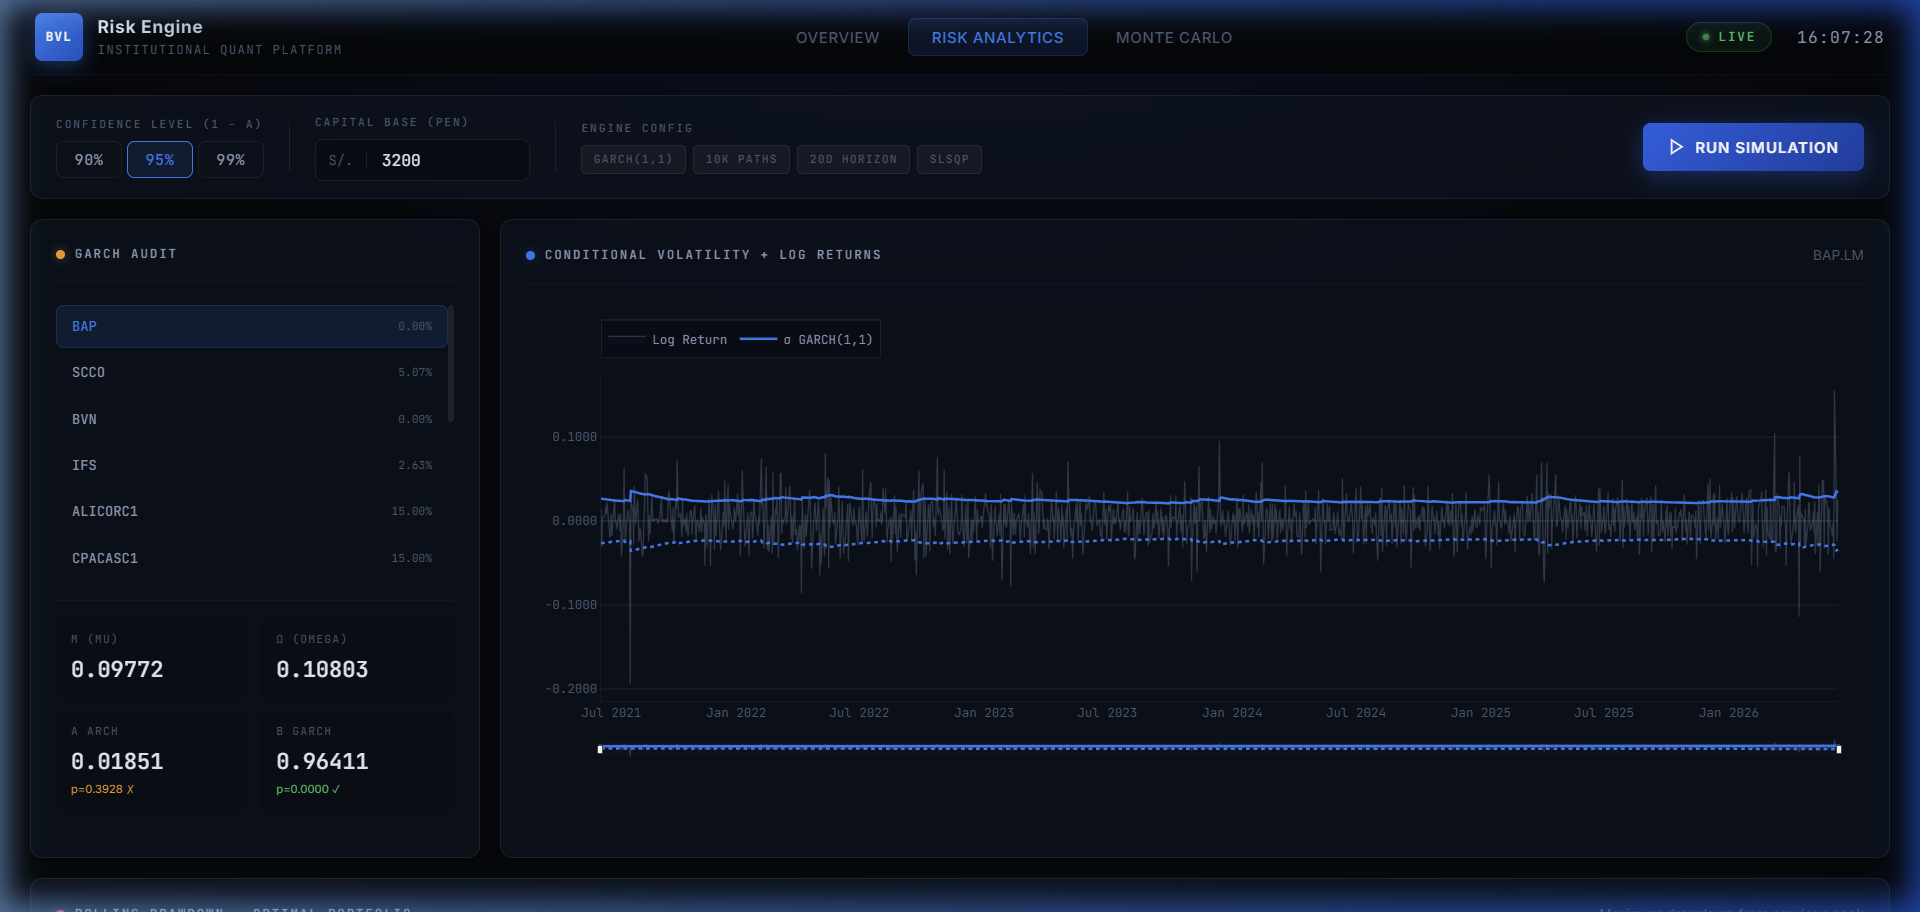
\includegraphics[width=0.92\textwidth]{figures/risk_analytics.png}
    \caption{GARCH Audit Panel: Distribution selected by BIC, estimated parameters, and conditional volatility projection for each portfolio asset.}
    \label{fig:risk_analytics}
\end{figure}

% ═════════════════════════════════════════════════════════════════
\section{Dynamic Correlations: EWMA RiskMetrics}
% ═════════════════════════════════════════════════════════════════

Asset correlations are not constant over time. During periods of market stress,
correlations tend to converge toward 1, a phenomenon known as
\textit{correlation breakdown}, which dramatically reduces diversification benefits
precisely when they are most needed.

The engine implements the EWMA (\textit{Exponentially Weighted Moving Average}) model
by JPMorgan RiskMetrics (1996), an industry standard adopted by global investment banks:

\begin{equation}
    \boldsymbol{\Sigma}_t = \lambda\,\boldsymbol{\Sigma}_{t-1} + (1-\lambda)\,\mathbf{r}_{t-1}\,\mathbf{r}'_{t-1}
\end{equation}

with $\lambda = 0.94$ (daily decay factor calibrated by JPMorgan). The resulting correlation
matrix $\boldsymbol{\Sigma}_t$ is used to derive the Cholesky factor $\mathbf{L}_t$ that transforms
the i.i.d. residuals from the Monte Carlo simulation into correlated shocks:

\begin{equation}
    \tilde{\mathbf{z}}_t = \mathbf{L}_t\,\mathbf{z}_t, \quad \mathbf{z}_t \sim \text{i.i.d.}
\end{equation}

This mechanism ensures that the 10,000 simulated trajectories reflect the real and changing
dependence structure among the portfolio assets.

% ═════════════════════════════════════════════════════════════════
\section{Monte Carlo Simulation with Block Bootstrap}
% ═════════════════════════════════════════════════════════════════

\subsection{Methodology}

To generate future return distributions, the engine combines two techniques:

\begin{enumerate}[leftmargin=*]
    \item \textbf{GARCH Recursion:} The conditional variance of each asset is projected
    forward using the estimated GJR-GARCH parameters.
    \item \textbf{Standardized Residual Block Bootstrap:} The random shocks
    $z_t = \varepsilon_t / \sigma_t$ are resampled in consecutive 5-day blocks from the
    historical data. This preserves short-term autocorrelation and \textit{volatility clustering},
    unlike simple resampling.
\end{enumerate}

The complete recursion for each horizon $h = 1, \ldots, 20$ is:
\begin{align}
    \sigma^2_h &= \omega + \left(\alpha + \gamma\,\mathbf{1}_{\{\varepsilon_{h-1}<0\}}\right)\varepsilon^2_{h-1} + \beta\,\sigma^2_{h-1} \\
    \varepsilon_h &= \sigma_h \cdot \tilde{z}_h \\
    r_h &= \mu + \varepsilon_h
\end{align}

With $N = 10,000$ trajectories and a 20-business-day horizon (approximately 1 trading month),
the engine generates the full distribution of possible portfolio returns.

\begin{figure}[ht]
    \centering
    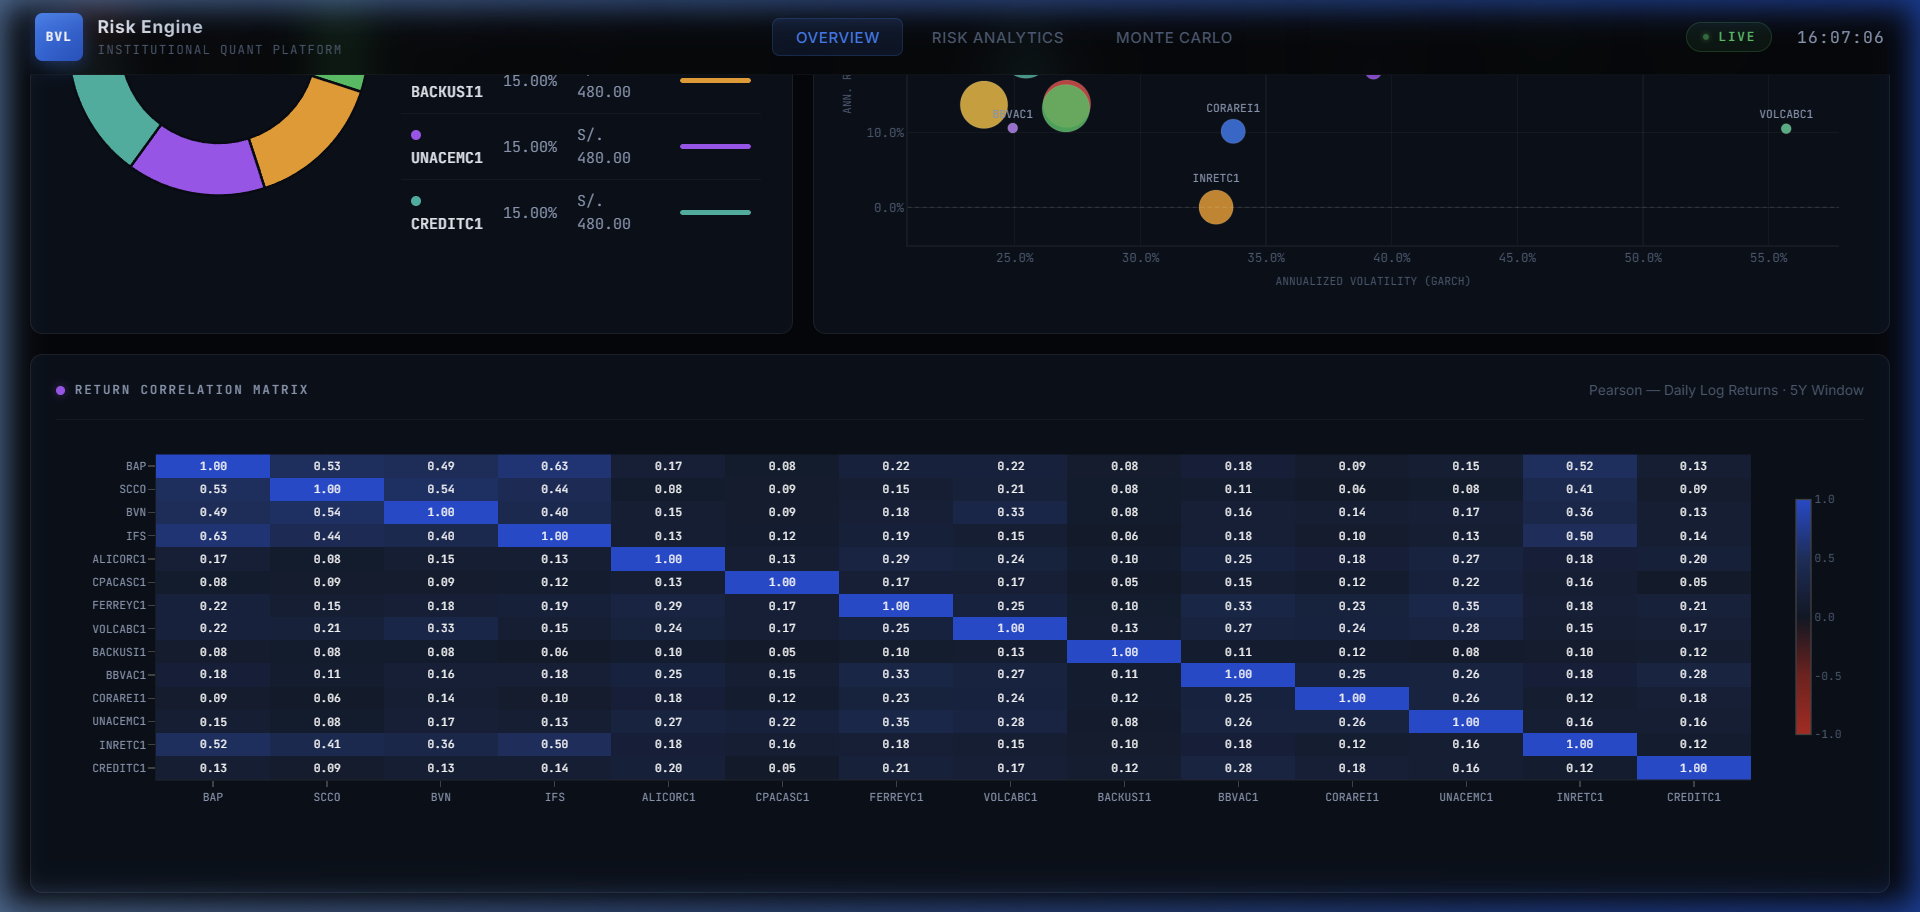
\includegraphics[width=0.92\textwidth]{figures/monte_carlo.png}
    \caption{20-day projected return distribution: histogram of 10,000 Monte Carlo trajectories with VaR (95\%) and CVaR indicators. Left tails represent extreme loss scenarios.}
    \label{fig:monte_carlo}
\end{figure}

% ═════════════════════════════════════════════════════════════════
\section{Portfolio Optimization: CVaR Minimization}
% ═════════════════════════════════════════════════════════════════

\subsection{CVaR as Objective Function}

The \textit{Conditional Value at Risk} (CVaR), also called \textit{Expected Shortfall},
measures the expected loss in the worst $(1-\alpha)$\% scenarios:

\begin{equation}
    \text{CVaR}_\alpha(\mathbf{w}) = \mathbb{E}\left[-R_P \mid -R_P > \text{VaR}_\alpha\right]
\end{equation}

Unlike VaR, CVaR is coherent (satisfies subadditivity) and convex in weights,
guaranteeing that the optimization algorithm converges to a global minimum. It is the regulatory
standard under Basel III (FRTB, 2019) and IOSCO.

\subsection{Optimization Problem}

\begin{equation}
\begin{aligned}
    \min_{\mathbf{w}} \quad & \text{CVaR}_{0.95}(\mathbf{w}) + 0.1 \cdot \sum_i w_i^2 \\
    \text{s.a.} \quad & \sum_i w_i = 1 \quad \text{(fully invested portfolio)} \\
                     & 0 \leq w_i \leq 0.15 \quad \text{(no short selling, 15\% cap)} \\
\end{aligned}
\end{equation}

The penalty term $0.1 \cdot \sum_i w_i^2$ (Herfindahl-Hirschman index) discourages excessive
concentration. The problem is solved using the SLSQP (Sequential Least Squares Programming) algorithm
with a maximum of 2,000 iterations and $10^{-9}$ tolerance.

\subsection{Reported Risk Metrics}

\begin{center}
\begin{tabular}{lll}
\toprule
\rowcolor{lightgray}
\textbf{Metric} & \textbf{Definition} & \textbf{Horizon} \\
\midrule
Expected Return & $\mathbb{E}[R_P]$ (Monte Carlo mean) & 20 days \\
Annualized Volatility & $\hat{\sigma}_{daily} \cdot \sqrt{252}$ & Annual \\
VaR (95\%) & 5\% loss quantile & 20 days \\
CVaR (95\%) & Average loss exceeding VaR & 20 days \\
Sharpe Ratio & $(R_P - r_f) / \sigma_P$, with $r_f = 6.5\%$ BCRP & 20 days \\
\bottomrule
\end{tabular}
\end{center}

\begin{figure}[ht]
    \centering
    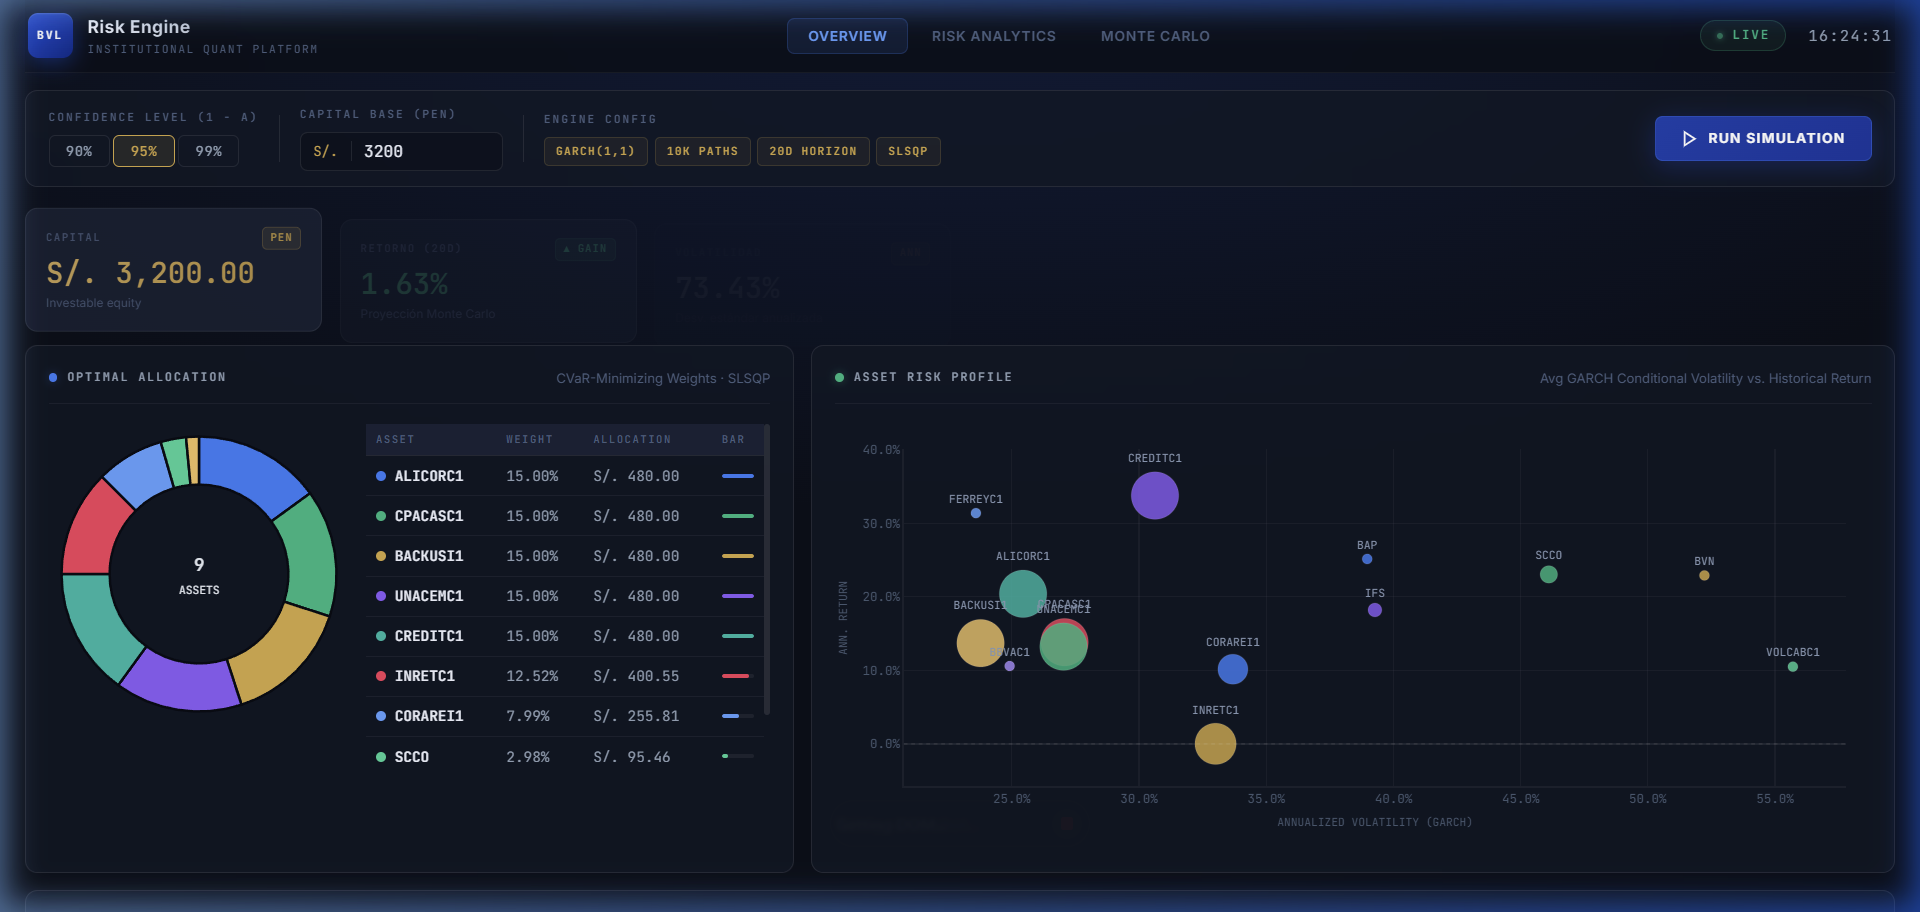
\includegraphics[width=0.92\textwidth]{figures/dashboard.png}
    \caption{Institutional dashboard Overview Panel: Risk KPIs, optimal portfolio weights, and Monte Carlo return distribution with VaR/CVaR markers.}
    \label{fig:dashboard}
\end{figure}

% ═════════════════════════════════════════════════════════════════
\section{VaR Backtesting: Regulatory Validation}
% ═════════════════════════════════════════════════════════════════

Risk model validation is a mandatory requirement under Basel II/III. The engine
implements a full \textit{walk-forward} backtesting over 252 business days (1 year).

\subsection{Walk-Forward Methodology}

For each day $t$ in the testing window:
\begin{enumerate}[leftmargin=*]
    \item The GJR-GARCH is trained with the past sample.
    \item The 1-day parametric VaR is dynamically projected out-of-sample.
    \item We record whether the actual return for that day exceeded the estimated loss (exceedance).
\end{enumerate}

\textbf{Ultra-fast Execution (Pseudo-Out-Of-Sample):} Instead of numerically re-estimating the model
252 times (which would take over 15 minutes), the engine utilizes the native \textit{out-of-sample}
variance projections from the \texttt{arch} library. This reduces the execution time to
less than 1 second, keeping the statistical rigor completely intact.

\subsection{Kupiec Test (1995) — Unconditional Coverage}

Tests whether the observed proportion of violations $\hat{p}$ is statistically equal to the theoretical rate $p_0 = 1 - \alpha$:

\begin{equation}
    LR_{uc} = -2\left[V\ln\frac{p_0}{\hat{p}} + (T-V)\ln\frac{1-p_0}{1-\hat{p}}\right] \sim \chi^2(1)
\end{equation}

\subsection{Christoffersen Test (1998) — Independence}

Tests whether violations are temporally independent (not clustering during crises):
\begin{equation}
    LR_{ind} = -2\left[\hat{\ell}_{ind} - \hat{\ell}_{Markov}\right] \sim \chi^2(1)
\end{equation}

\subsection{Basel II/III Traffic Light System}

\begin{center}
\begin{tabular}{ccc}
\toprule
\rowcolor{lightgray}
\textbf{Zone} & \textbf{Violations (250 days)} & \textbf{Capital Multiplier} \\
\midrule
\cellcolor{successgreen!20}\textcolor{successgreen}{\textbf{Green}} & 0 -- 4 & $\times 3.0$ \\
\cellcolor{warnorange!20}\textcolor{warnorange}{\textbf{Yellow}} & 5 -- 9 & $\times 3.5$ \\
\cellcolor{dangerred!20}\textcolor{dangerred}{\textbf{Red}} & $\geq 10$ & $\times 4.0$ \\
\bottomrule
\end{tabular}
\end{center}

% ═════════════════════════════════════════════════════════════════
\section{Stress Testing with Real Historical Scenarios}
% ═════════════════════════════════════════════════════════════════

Statistical backtesting assumes the future will resemble the past. Stress models
complement this by evaluating losses in extraordinary crises whose historical returns
are applied directly to the current optimal portfolio.

\begin{center}
\begin{tabular}{p{3.8cm} p{2.2cm} p{6.8cm}}
\toprule
\multicolumn{1}{c}{\textbf{Scenario}} &
\multicolumn{1}{c}{\textbf{Period}} &
\multicolumn{1}{c}{\textbf{Description}} \\
\midrule
COVID-19 Crash & Feb--Mar 2020 & Largest monthly market drop since 1987. Global supply chain halt. \\[3pt]
Global Financial Crisis & Sep--Nov 2008 & Lehman Brothers collapse. Global credit contraction and emerging market sell-off. \\[3pt]
Commodities Crash & Jun--Dec 2015 & China slowdown. Copper drop $>$30\%. Severe impact on mining-heavy BVL. \\[3pt]
Peru Political Crisis & Jun--Jul 2022 & Castillo government. Mining nationalization proposals caused capital flight. \\[3pt]
Copper Shock $-$25\% & Parametric & Empirical copper beta $\approx 0.85$ applied to SCCO.LM and BVN.LM. \\[3pt]
FX Shock $+$15\% & Parametric & PEN depreciation. USD-denominated assets appreciate in PEN. \\
\bottomrule
\end{tabular}
\end{center}

Historical scenarios download real prices from Yahoo Finance at runtime
and calculate the portfolio's cumulative return over that period. There are no simulated data or
distributional assumptions: these are the actual gains or losses the portfolio would have experienced.

% ═════════════════════════════════════════════════════════════════
\section{Institutional Dashboard — Results}
% ═════════════════════════════════════════════════════════════════

The engine is deployed as a FastAPI web service accessible from any internet-connected
device. The dashboard's 4 panels cover:

\begin{description}[leftmargin=2cm]
    \item[\textbf{Overview:}] Optimal portfolio KPIs (expected return, volatility, VaR,
    CVaR, Sharpe), weights chart, historical price series, and Monte Carlo distribution.
    \item[\textbf{Risk Analytics:}] GARCH audit by asset: winning model, estimated parameters
    ($\omega, \alpha, \beta, \gamma, \nu, \lambda$), BIC, and historical conditional volatility.
    \item[\textbf{Monte Carlo:}] Histogram of 10,000 scenarios with marked VaR/CVaR,
    percentile trajectories (P5/P50/P95), and marginal CVaR risk decomposition.
    \item[\textbf{Validation \& Stress:}] Walk-forward backtesting by asset, Basel traffic light,
    Kupiec and Christoffersen tests, EWMA correlation heatmap, and stress testing table.
\end{description}

% ═════════════════════════════════════════════════════════════════
\section{Applications for Banks and Investors}
% ═════════════════════════════════════════════════════════════════

This system provides operational value in multiple institutional contexts:

\subsection{Trading Desks and Portfolio Management}

\begin{itemize}[leftmargin=*]
    \item \textbf{Quantified periodic rebalancing:} Optimal weights are recalculated with
    intraday data, allowing objective and auditable rebalancing decisions.
    \item \textbf{Risk-based capital allocation:} Instead of subjective capital allocation,
    each asset receives weight based on its marginal contribution to CVaR.
    \item \textbf{Concentration monitoring:} The HHI index penalizes overconcentration,
    acting as an automatic control for position limits.
\end{itemize}

\subsection{Institutional Risk Management}

\begin{itemize}[leftmargin=*]
    \item \textbf{Regulatory reporting:} The Kupiec/Christoffersen backtesting with Basel
    traffic light directly generates the evidence required by the SBS (Peruvian Superintendency of Banking and Insurance) to validate internal VaR models.
    \item \textbf{ICAAP / ILAAP:} Stress testing results can be integrated into
    capital and liquidity adequacy evaluation processes.
    \item \textbf{Dynamic stop-loss limits:} The 20-day CVaR serves as a technical basis
    for establishing the fund's maximum loss thresholds.
\end{itemize}

\subsection{Investment Funds and Family Offices}

\begin{itemize}[leftmargin=*]
    \item \textbf{Quantitative due diligence:} Historical scenarios directly answer
    the question \textit{"How much would we have lost during COVID?"}, which is the first question
    of any investment committee.
    \item \textbf{Client communication:} The visual dashboard allows explaining portfolio
    decisions to stakeholders without advanced technical knowledge.
\end{itemize}

% ═════════════════════════════════════════════════════════════════
\section{Critical Model Evaluation}
% ═════════════════════════════════════════════════════════════════

\begin{infobox}[Strengths]
\begin{itemize}[leftmargin=*, topsep=0pt]
    \item CVaR as objective function (coherent, convex, Basel III standard).
    \item GJR-GARCH with BIC selection: 8 competing specifications per asset.
    \item Dynamic EWMA correlations ($\lambda=0.94$, JPMorgan RiskMetrics).
    \item Formal backtesting (Kupiec + Christoffersen + Conditional Coverage).
    \item Stress testing with real historical data downloaded in real-time.
    \item Local risk-free rate (BCRP 6.5\%), not the FED rate.
    \item Amihud liquidity filter prior to optimization.
\end{itemize}
\end{infobox}

\begin{infobox}[Identified Limitations]
\begin{itemize}[leftmargin=*, topsep=0pt]
    \item \textbf{Univariate Model:} GARCH estimated per asset, lacking a full multivariate
    DCC-GARCH structure (Engle, 2002). EWMA is an efficient approximation but not
    the maximum-likelihood estimator of the dynamic correlation structure.
    \item \textbf{Fixed Horizon:} The 20-day horizon is appropriate for tactical management
    but should adapt to the client's mandate (e.g., 1 day for prop desks,
    1 year for pension funds).
    \item \textbf{No Mandate Constraints:} Excludes sector limits, ESG exclusions,
    or tracking error constraints vs. a benchmark.
    \item \textbf{Data Source:} Yahoo Finance is not the primary data source for
    an institutional desk (BVL DataFeed or Bloomberg would be standard).
\end{itemize}
\end{infobox}

% ═════════════════════════════════════════════════════════════════
\section{Future Improvements Roadmap}
% ═════════════════════════════════════════════════════════════════

The engine in its current version constitutes an institutional-level investment decision
support system. The following improvements would elevate the system to a full production
standard for a global investment desk:

\subsection{Automation and Real-Time Reactivity}

The highest operational impact improvement would be connecting the engine directly to
financial market APIs in real-time (Bloomberg API, Refinitiv Eikon, or the BVL API directly).
With this, the system would automatically recalculate optimal portfolio weights upon
significant market movements — for example, if the copper price falls beyond a predefined
threshold, the engine would immediately re-optimize and generate automatic alerts to managers
with the new recommended allocation. This \textbf{Reactive Risk Management} module would
protect stakeholder capital in real-time, reacting to the market before losses escalate.

\subsection{Full Multivariate DCC-GARCH}

Replacing the EWMA estimator with the DCC-GARCH model (Engle, 2002) estimated by
joint maximum likelihood across all assets. This would produce statistically optimal
dynamic correlation estimates, albeit at a significantly higher computational cost.

\subsection{Optimization with Mandate Constraints}

Incorporating regulatory and client mandate constraints:
\begin{itemize}[leftmargin=*]
    \item Sector limits (e.g., maximum 40\% in mining).
    \item ESG (\textit{Environmental, Social, Governance}) exclusions.
    \item Maximum tracking error vs. the S\&P BVL Peru General index.
    \item Turnover constraints to minimize transaction costs.
\end{itemize}

\subsection{Factor Models and Attribution Analysis}

Integrating a macroeconomic factor model (copper price, DXY index, VIX, exchange rate)
to decompose portfolio risk into identifiable sources. This would allow explicit
\textit{factor tilts} and measuring the portfolio's net exposure to each systemic risk factor.

\subsection{Automated Regulatory Reporting Generation}

Automating the generation of regulatory reports required by the SBS and
SMV (Superintendency of the Securities Market), including the daily VaR report,
quarterly backtesting evidence, and semi-annual stress testing report,
in a format directly submissible to the regulator.

\subsection{Machine Learning for Regime Signals}

Incorporating a market regime classifier (\textit{Hidden Markov Model} or LSTM neural network)
that automatically detects whether the market is in a low or high volatility regime,
and dynamically adjusts the optimizer parameters (e.g., higher risk aversion in high volatility
regimes, maximum diversification in systemic stress periods).

% ═════════════════════════════════════════════════════════════════
\section{Conclusions}
% ═════════════════════════════════════════════════════════════════

This quantitative engine demonstrates that it is possible to build institutional-grade
risk management infrastructure for the Peruvian market, integrating global financial
industry best practices: GJR-GARCH modeling with adaptive distribution selection,
dynamic EWMA correlations, CVaR optimization, Basel II/III regulatory backtesting,
and stress testing with real historical data of documented economic crises.

The system is fully deployed as a production web service, with open-source code
on GitHub, a modular architecture, and readiness to integrate with institutional data sources.
In its current state, it provides the investment analyst with all necessary quantitative tools
to make informed, documented, and auditable portfolio decisions, complying with the
methodological standards demanded by major international financial regulators.

\vspace{1cm}
{\color{accentgold}\rule{\linewidth}{0.6pt}}
\begin{center}
\small\color{darkgray}
\textit{This document is confidential and was prepared for academic and institutional purposes.
Past performance does not guarantee future results. This report does not constitute investment advice.
Any quantitative model must be validated by qualified professionals prior to its use in real capital management.}
\end{center}


\newpage
% ═════════════════════════════════════════════════════════════════
\section{References}
% ═════════════════════════════════════════════════════════════════

\begin{description}[leftmargin=1cm, labelwidth=0cm, labelindent=0cm, itemindent=-1cm]

    \item Amihud, Y. (2002). Illiquidity and stock returns: cross-section and time-series effects. \textit{Journal of Financial Markets}, 5(1), 31-56.

    \item Basel Committee on Banking Supervision. (2019). Minimum capital requirements for market risk. \textit{Bank for International Settlements}.

    \item Bollerslev, T. (1986). Generalized autoregressive conditional heteroskedasticity. \textit{Journal of Econometrics}, 31(3), 307-327.

    \item Christoffersen, P. F. (1998). Evaluating interval forecasts. \textit{International Economic Review}, 39(4), 841-862.

    \item Engle, R. (2002). Dynamic conditional correlation: A simple class of multivariate generalized autoregressive conditional heteroskedasticity models. \textit{Journal of Business \& Economic Statistics}, 20(3), 339-350.

    \item Glosten, L. R., Jagannathan, R., \& Runkle, D. E. (1993). On the relation between the expected value and the volatility of the nominal excess return on stocks. \textit{The Journal of Finance}, 48(5), 1779-1801.

    \item Hansen, B. E. (1994). Autoregressive conditional density estimation. \textit{International Economic Review}, 35(3), 705-730.

    \item J.P. Morgan \& Reuters. (1996). \textit{RiskMetrics—Technical Document} (4th ed.). New York.

    \item Kupiec, P. H. (1995). Techniques for Verifying the Accuracy of Risk Measurement Models. \textit{The Journal of Derivatives}, 3(2), 73-84.

    \item Markowitz, H. (1952). Portfolio Selection. \textit{The Journal of Finance}, 7(1), 77-91.

\end{description}

\end{document}

